\section{Dynamic Models}

\subsection{Use Case Sequence Diagrams}
\subsubsection{CreateSale Sequence Diagram}
\begin{figure}[H]
	\centering
		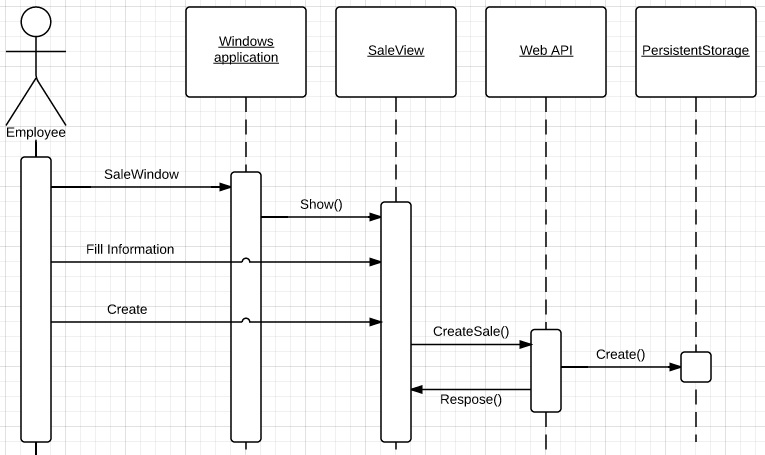
\includegraphics[width=\textwidth]{Figures/SequenceDiagram-CreateSale}\\
		% place the figure in the Figures folder (located with the main file)
		% you need to fix the scale a few times to get it right, but latex does not compress so one can always zoom in to see details.
	\caption{Sequence diagram of the CreateSale use case.}
  \label{fig:SequenceDiagram-CreateSale}
  % label it something meanfull
\end{figure}

Sequence diagram \ref{fig:SequenceDiagram-CreateSale} is made from the use case \texttt{CreateSale UC-1: \ref{create-order-use-case}}. \\\\
In this use case, the employee starts with opening the \texttt{DriveIT Windows Client}, and thereafter navigates to the \texttt{Sale} view. In the \texttt{Sale} view, the employee fills in the information necessary to create a \texttt{Sale}, and after the \texttt{Employee} has finished filling in the information, he or she clicks on the "Create" button.

The sale will then be created and saved in the persistent storage. The \texttt{Employee} will then be prompted with a pop-up window, telling if the save was a success or an error has occurred.

\subsubsection{CreateUserAccount Sequence Diagram}
\begin{figure}[H]
	\centering
		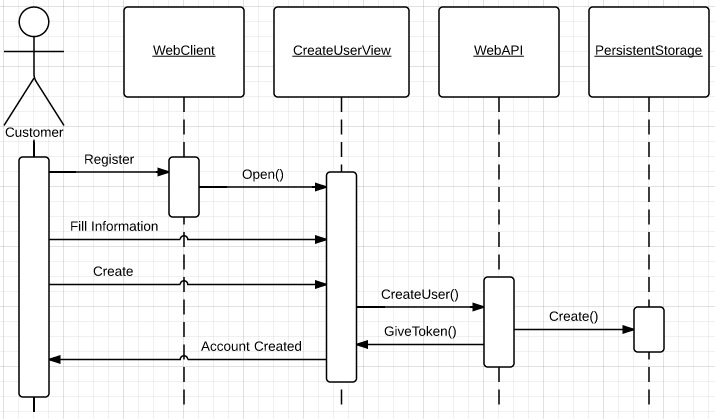
\includegraphics[width=\textwidth]{Figures/SequenceDiagram-CreateUserAccount}\\
		% place the figure in the Figures folder (located with the main file)
		% you need to fix the scale a few times to get it right, but latex does not compress so one can always zoom in to see details.
	\caption{Sequence diagram of the CreateUserAccount use case.}
  \label{fig:SequenceDiagram-CreateUserAccount}
  % label it something meanfull
\end{figure}

Sequence diagram \ref{fig:SequenceDiagram-CreateUserAccount} is made from the use case \texttt{CreateUserAccount UC-2: \ref{create-account-use-case}}. \\\\
In this use case, the non-registered \texttt{Customer} has navigated to the \texttt{DriveIT Web Client} and thereafter clicks "Register", whereafter the customer is directed to the CreateUserWindow. 

In this window, the user will be filling in the necessary information, and after the \texttt{Customer} has finished filling in the information, he or she click on the "Create" button and the user account will then be created and saved in the persistent storage. The CreateUserWindow will then show that the creation of the user accout has been a success, and the customer can then log in into the \texttt{DriveIT Web Client}.

\subsubsection{ContactInterestedCustomer Sequence Diagram}
\begin{figure}[H]
	\centering
		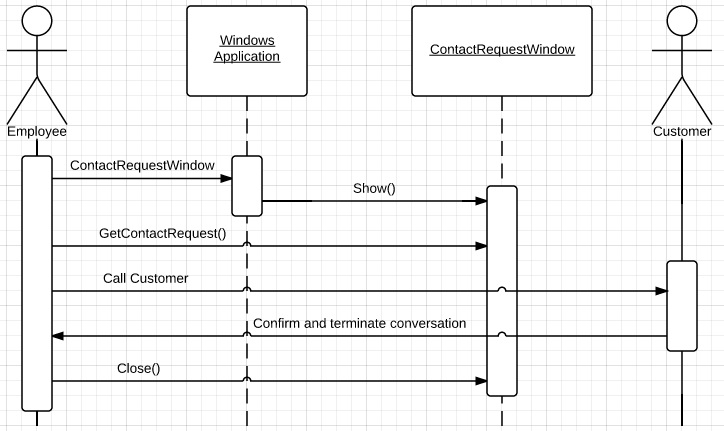
\includegraphics[width=\textwidth]{Figures/SequenceDiagram-ContactInterestedCustomer}\\
		% place the figure in the Figures folder (located with the main file)
		% you need to fix the scale a few times to get it right, but latex does not compress so one can always zoom in to see details.
	\caption{Sequence diagram of the ContactInterestedCustomer use case.}
  \label{fig:SequenceDiagram-ContactInterestedCustomer}
  % label it something meanfull
\end{figure}

Sequence diagram \ref{fig:SequenceDiagram-ContactInterestedCustomer} is made from the use case \texttt{ ContactInterestedCustomer UC-3: \ref{create-car-use-case}}. \\\\
In this case, the employee starts with opening the windows application. The employee then navigates to the ContactRequestWindow, where there will be shown a list of contact requests by different customers. The employee picks one of the contact requests and a more detailed view of the contact request will be shown. The employee then calls the customer, starts a conversation regarding the contact request, and after a while the customer will confirm his or her choice and terminate the conversation. The employee will then close the contact request detail window and create a sale.

\subsubsection{RequestEmployeeContact Sequence Diagram}
\begin{figure}[H]
	\centering
		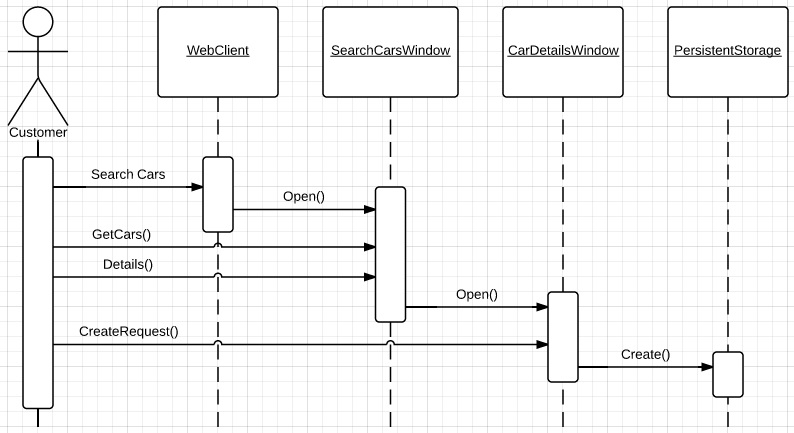
\includegraphics[width=\textwidth]{Figures/SequenceDiagram-RequestEmployeeContact}\\
		% place the figure in the Figures folder (located with the main file)
		% you need to fix the scale a few times to get it right, but latex does not compress so one can always zoom in to see details.
	\caption{Sequence diagram of the RequestEmployeeContact use case.}
  \label{fig:SequenceDiagram-RequestEmployeeContact}
  % label it something meanfull
\end{figure}

Sequence diagram \ref{fig:SequenceDiagram-RequestEmployeeContact} is made from the use case \texttt{ RequestEmployeeContact UC-4: \ref{request-contact-use-case}}. \\\\
In this case, the customer, non-registered or registered and logged on, has navigated to our web client and thereafter click "Find Cars", and thereafter the search cars window will show. The customer will then search for the specific car that he or she are trying to find. The customer will then navigate to details of the car, by clicking "Details" and then create a request, by clicking "Create Request", whereas the contact request then will created and saved in the persistent storage.

\subsection{State Diagrams}
\begin{figure}[H]
	\centering
		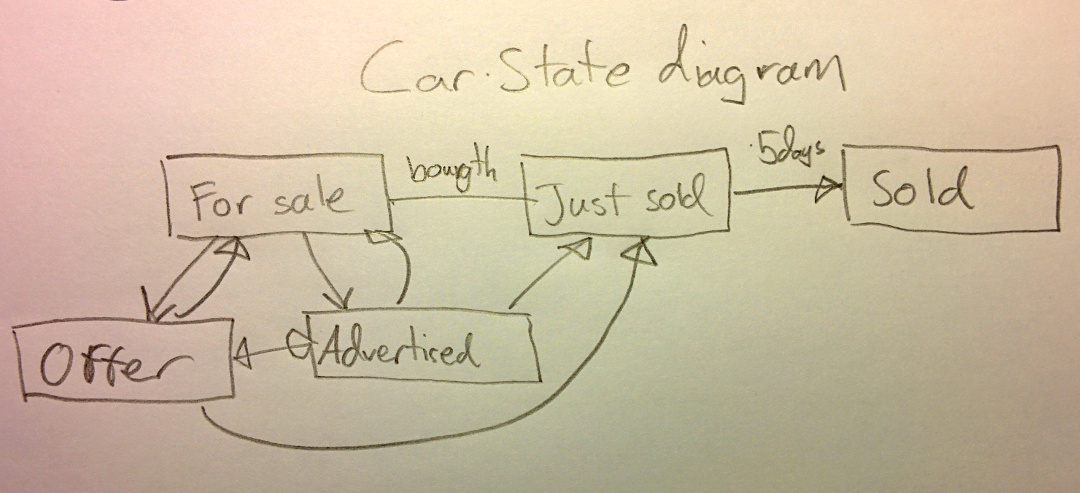
\includegraphics[width=\textwidth]{Figures/StateDiagram-Car}\\
		% place the figure in the Figures folder (located with the main file)
		% you need to fix the scale a few times to get it right, but latex does not compress so one can always zoom in to see details.
	\caption{State diagram of the Car object}
  \label{fig:StateDiagram-Car}
\end{figure}
The \ref{fig:StateDiagram-Car} shows the states a car entity can be in. The car should always be possible to delete as shown in the diagram, but to be sold the car must first enter the \emph{For Sale} state. In the \emph{For Sale} and \emph{Sold} state the car should be visible from the \texttt{DriveIT Web Client} with a label indicating which of the two states its in, and the car should be visible from the \texttt{DriveIT Windows Client} in all its states.\\
\begin{figure}[H]
	\centering
		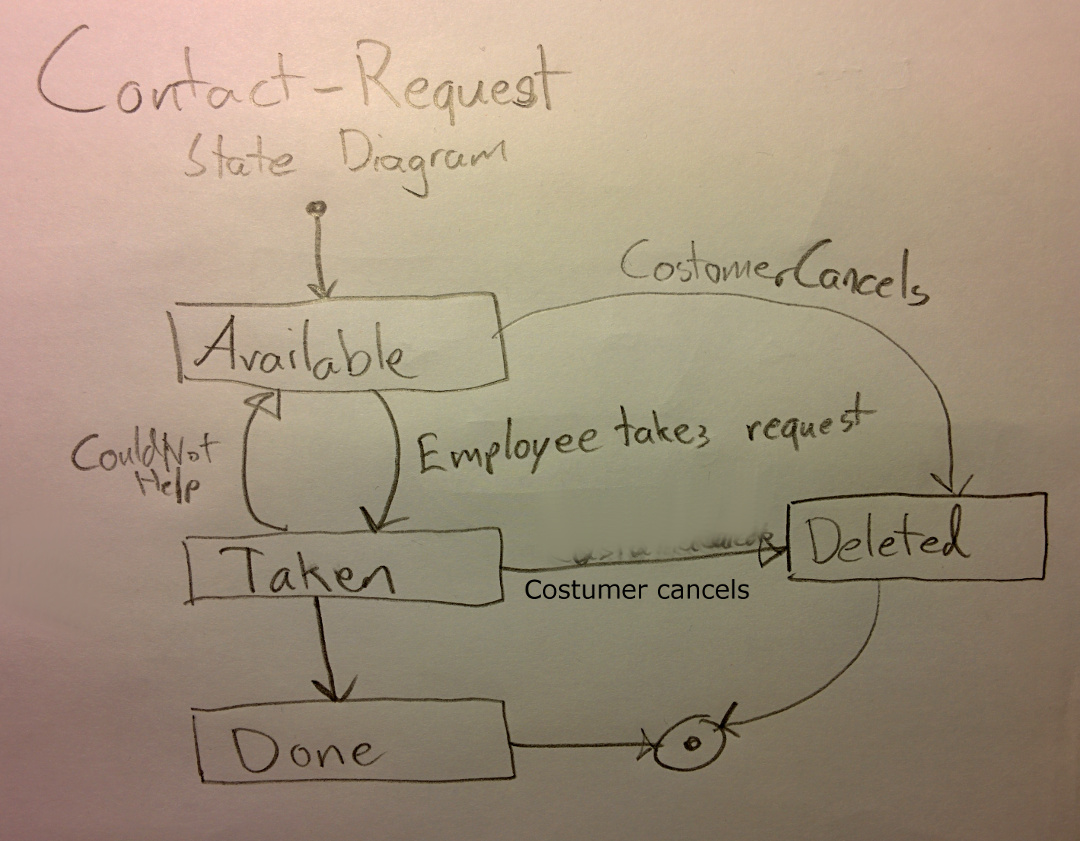
\includegraphics[width=\textwidth]{Figures/StateDiagram-ContactRequest}\\
		% place the figure in the Figures folder (located with the main file)
		% you need to fix the scale a few times to get it right, but latex does not compress so one can always zoom in to see details.
	\caption{State diagram of the ContactRequest object}
  \label{fig:StateDiagram-ContactRequest}
  % label it something meanfull
\end{figure}